\documentclass[10pt,twocolumn]{article}

\usepackage[margin=0.72in]{geometry}
\usepackage{times}
\usepackage{microtype}
\usepackage{booktabs}
\usepackage{graphicx}
\usepackage{amsmath}
\usepackage[numbers,sort&compress]{natbib}
\usepackage[hidelinks]{hyperref}
\usepackage{xcolor}
\usepackage{capt-of}
\usepackage{placeins}

\setlength{\columnsep}{0.28in}
\setlength{\abovecaptionskip}{6pt}
\setlength{\belowcaptionskip}{2pt}
\renewcommand{\bibsection}{\section*{References}}
\bibliographystyle{plainnat}

% Replace these two commands before submission. The repository does not record either value.
\newcommand{\paperauthor}{[Author name]}
\newcommand{\paperaffil}{[Author affiliation]}

\title{A Shared Byte-Level BPE Vocabulary Uses More Held-Out Tokens than Dedicated Vocabularies: An English--Hindi--Nepali Study}
\author{\paperauthor\\
{\paperaffil}\thanks{Replace \texttt{\string\paperauthor} and \texttt{\string\paperaffil} in the preamble. The repository does not record an author name or affiliation.}}
\date{}

\begin{document}
\maketitle

\begin{abstract}
We compare dedicated and fully shared byte-level byte-pair encoding (BPE) vocabularies for English, Hindi, and Nepali under a small, fixed vocabulary.
The comparison is intrinsic: the outcome is the number of tokens required to encode a fixed held-out text, together with exact encode--decode reconstruction.
At a requested vocabulary of 1{,}024, three resampled training selections of about 300{,}000 UTF-8 bytes per language give mean shared-vocabulary token-count penalties of 14.22\%, 15.62\%, and 18.61\% for English, Hindi, and Nepali.
A second regime draws dedicated and joint models from the same per-language subsets of about 100{,}000 bytes, so the joint model trains on about 300{,}000 bytes in total.
The penalty remains positive in all nine language--replicate comparisons, with means of 12.52\%, 13.08\%, and 16.19\%.
Those smaller percentages coincide with higher absolute token counts for both dedicated and joint models.
The two regimes change sample size and document composition together, so the difference is not an effect of training-data quantity alone.
Sample standard deviations describe overlapping resamples and are not significance tests.
The result is a reproducible case study for this corpus and implementation, not a general claim about multilingual tokenization or downstream model quality.
\end{abstract}

\section{Introduction}

Multilingual models often use one vocabulary for every language they serve.
A joint tokenizer learns its merges from the combined training distribution.
A dedicated tokenizer learns its merges from one language's distribution.
One possible consequence is that some joint merges reflect cross-lingual co-occurrence and contribute less to shortening a single language's encoding.
That account is a possible explanation.
This study does not establish it.
The measured question is whether a joint vocabulary uses more tokens on held-out text, which is separate from whether shared tokens help a downstream task.

This paper asks three questions about a deterministic byte-level BPE implementation and one English--Hindi--Nepali web sample.
\begin{enumerate}
\item When each language contributes about the same amount of training text and the requested vocabulary is 1{,}024, does a joint vocabulary encode held-out text with more tokens than a vocabulary trained on that language alone?
\item Does a positive penalty remain when the joint model and the dedicated models are trained on the same per-language documents, so the joint training text is about one-third as large?
\item In one balanced selection, is the penalty positive at requested sizes 512, 1{,}024, and 2{,}048?
\end{enumerate}
The first question holds per-language training text approximately fixed and therefore gives the joint model about three times as much text.
The second holds the source documents fixed between the dedicated and joint conditions within each replicate.
Neither question is a causal experiment that changes only the joint model's byte budget.

We do not present byte-level BPE, shared vocabularies, vocabulary allocation, or Indic tokenization as new methods.
The contribution is a small, fully specified comparison with saved hashes, exact reconstruction checks, and two budget regimes that are reported separately.
Hindi and Nepali share Devanagari in this sample.
A positive penalty under that pairing means that shared script, by itself, did not produce a shorter encoding here.
It does not show that script sharing is generally harmful, and it does not measure transfer.

\section{Related work}

Byte-pair encoding was introduced for open-vocabulary neural machine translation by merging frequent character sequences \citep{sennrich-etal-2016-neural}.
Our trainer applies that merge rule to UTF-8 bytes.
The implementation is a research reimplementation with an explicit left-to-right tie break.
It is not offered as a new algorithm.

Work on multilingual vocabularies has treated capacity allocation as a modeling choice rather than as a settled benefit of sharing.
Clustered vocabularies can improve TyDi QA, XNLI, and WikiAnn NER without a larger model or more data \citep{chung-etal-2020-improving}.
VoCap assigns vocabulary capacity by language for cross-lingual pre-training \citep{zheng-etal-2021-allocating}.
XLM-V argues that a single shared vocabulary can bottleneck multilingual masked language models when capacity is not allocated to languages with little lexical overlap \citep{liang-etal-2023-xlm}.
Those papers evaluate downstream tasks at a scale this study does not approach.
We use them to locate the question, not to claim the same findings.

Vocabulary overlap itself has task-dependent reported effects.
\citet{limisiewicz-etal-2023-tokenization} find that overlap can hurt part-of-speech tagging and dependency-label labeling while helping named-entity recognition and sentence-level tasks.
\citet{patil-etal-2022-overlap} report that encouraging overlap among related languages can improve zero-shot transfer into low-web-resource languages.
Our metric cannot decide between those downstream patterns.
A higher intrinsic token count is compatible with either better or worse task performance.

For Indian languages, \citet{brahma-etal-2026-multilingual} study 17 languages, BPE and Unigram LM, normalization, vocabulary size, and joint versus cluster construction.
Their abstract reports gains from script-specific normalization and from cluster-based construction on downstream tasks, and better morphological boundary retention for Unigram LM than for BPE.
That study is the closer neighbor of this paper.
Ours is narrower: three languages, one byte-level BPE implementation, no Unigram LM condition, no cluster vocabulary, and no downstream model.
\citet{ali-etal-2024-tokenizer} report that fertility and parity do not always predict downstream behavior of 2.6B-parameter models.
We therefore treat token count as the measured outcome and stop there.

\section{Data}

\subsection{Source and split}

The saved manifest names the Hugging Face dataset \texttt{ashtok897/indic-hplt-v2}, streamed from its \texttt{train} split on 28 October 2026 \citep{mahajan-2026-indic-hplt}.
The Mahajan citation is the one requested by the dataset card retrieved on 29 October 2026.
It is a dataset-card citation, not a peer-reviewed paper.
That card describes the release as text derived from HPLT monolingual v3 and points to HPLT~3.0, which is cited here as the arXiv preprint arXiv:2511.01066 \citep{oepen-etal-2025-hplt}.
This repository stores no dataset revision, commit, or snapshot hash.
A later copy of the card is not evidence that the stream of 28 October 2026 had the same contents or the same documentation.
The files under \texttt{data/processed/} are the corpus of record.

Collection kept English (\texttt{en}), Hindi (\texttt{hi}), and Nepali (\texttt{ne}).
Null bytes were replaced, whitespace was collapsed, and strings were stripped.
Texts shorter than 100 characters or longer than 20{,}000 characters were rejected.
Exact duplicates of the cleaned text were removed within each language.
Collection stopped at 1{,}000{,}000 code points per language, using Python's \texttt{len}, not UTF-8 bytes.
The saved pool contains 102 English documents, 451 Hindi documents, and 538 Nepali documents.

The train/test cut shuffles with \texttt{random.Random(42)} and assigns the last 10\% of documents, by count, to test.
One generator continues from English through Hindi to Nepali, so the three shuffles are coupled.
The split is not a 10\% byte split.
Table~\ref{tab:pool} records the result.
In the later selectors, one document is one nonempty stripped line.

\begin{center}
\small
\begin{tabular}{@{}lrrr@{}}
\toprule
 & English & Hindi & Nepali \\
\midrule
Pool documents & 102 & 451 & 538 \\
Train documents & 91 & 405 & 484 \\
Test documents & 11 & 46 & 54 \\
Test UTF-8 bytes & 93{,}262 & 226{,}287 & 295{,}837 \\
\bottomrule
\end{tabular}
\captionof{table}{Saved pool after the 28 October 2026 collection. Test byte counts are the held-out files used by every controlled experiment.}
\label{tab:pool}
\end{center}

\subsection{What the audit does and does not show}

A saved audit found no exact stripped-line overlap between processed train and test text for any pair of these languages, no within-file duplicate lines in the processed splits or the 300{,}000-byte resamples, and no NFC or NFKC collisions in those files.
Character-shingle screening at Jaccard threshold 0.90 and shingle size 5 found no candidate pairs in the same files.
The audit states that this screening does not detect paraphrases.
It also states that file hashes do not establish upstream provenance and that the audit cannot show the test set is free of contamination created before this split.
We did not audit personally identifiable information.

\section{Tokenizer}

The controlled experiments use one implementation.
Training encodes text as UTF-8 bytes.
The base vocabulary is the 256 byte values.
A requested size $V$ schedules $V-256$ merges.
The stored vocabulary size is 256 plus the number of merges completed.
Every controlled model in this study reached its requested size, so the 512, 1{,}024, and 2{,}048 models contain 256, 768, and 1{,}792 merges.

Each step merges the most frequent adjacent pair in the current training sequence.
If several pairs share that count, the implementation keeps the pair inserted first while scanning left to right.
Encoding then applies the earliest learned merge that is still present, and repeats.
Decoding concatenates the stored byte strings and decodes UTF-8 with replacement on invalid sequences.
Exact reconstruction means the decoded string equals the original string.
There is no random seed inside the BPE loop.
Given the training bytes, the merges are determined.

A separate full-corpus run at requested size 4{,}096 compares this byte-level tokenizer with grapheme and akshara variants.
That run is a contextual baseline in the results table and is not one of the three evidence tiers below.
The grapheme and akshara code is not used for the shared-versus-dedicated claims.

\section{Experimental design}

\subsection{Conditions}

A dedicated model is trained on one language.
A joint model is trained on the concatenation of the three language strings for that condition, joined by a newline.
Each language file already ends in a newline, so the joint string is two bytes longer than the sum of the three files.
All joint and dedicated models in a comparison use the same requested vocabulary.
The match is the vocabulary size of each tokenizer.
It is not a match of aggregate vocabulary capacity.
At requested size 1{,}024, the shared condition is one vocabulary of 1{,}024 entries, while the three dedicated tokenizers together contain 3{,}072 entries.
The single-run sizes 512 and 2{,}048 follow the same per-tokenizer rule, so the three dedicated vocabularies together contain 1{,}536 and 6{,}144 entries at those sizes.
No saved condition gives the joint vocabulary as many entries as the three dedicated vocabularies combined.
The results characterize this per-tokenizer comparison.
They do not isolate the effect of sharing under an equal aggregate vocabulary budget, and that alternative comparison was not run.
Evaluation uses the same held-out file for a language in every tier.
Dedicated models are scored on their own language.
The joint model is scored on each language separately.

The token-count penalty is
\begin{equation}
100 \times \frac{T_{\text{joint}} - T_{\text{dedicated}}}{T_{\text{dedicated}}},
\label{eq:penalty}
\end{equation}
where $T$ is the number of token ids on the held-out text.
A positive value means the joint vocabulary uses more tokens.
For three replicates we report the arithmetic mean and the sample standard deviation, with divisor $n-1$.
These three resamples share documents, so the standard deviation describes that spread.
It is not a confidence interval, and we report no hypothesis test.

\subsection{Three evidence tiers}

The tiers answer different questions and use different selections.

\paragraph{Single-run sweep.}
One deterministic selection keeps complete lines from each processed training file, ordered by the SHA-256 of the line, under a 300{,}000-byte cap.
That selector counts document bytes and does not count separator newlines toward the cap.
The written files contain 297{,}381 English bytes, 299{,}885 Hindi bytes, and 299{,}348 Nepali bytes.
The joint model trains on 896{,}616 bytes.
We train requested sizes 512, 1{,}024, and 2{,}048 once each.
A second saved 1{,}024 run uses the same training hashes and the same test-token counts.
It is the same selection, not a replicate.
This tier has no sample standard deviation.

\paragraph{Fixed per-language text.}
Three selections use seeds 11, 22, and 33.
Lines of the processed training file are ordered by the SHA-256 of the seed, a colon, and the line.
Whole lines are kept while the file, including newlines, stays within 300{,}000 UTF-8 bytes.
Each dedicated model therefore trains on about 300{,}000 bytes of one language.
The joint model trains on all three files.
Its saved sizes are 896{,}306, 895{,}182, and 899{,}404 bytes, against dedicated sums of 896{,}304, 895{,}180, and 899{,}402.
``About 900 KB'' in prose is a decimal approximation of these integers, not a count in kibibytes.
Every line in these resamples occurs in the corresponding processed training file.
Document Jaccard between resample pairs is 0.140--0.231 for English, 0.066--0.087 for Hindi, and 0.047--0.103 for Nepali.
Rounded to two decimals, those spans are 0.14--0.23, 0.07--0.09, and 0.05--0.10.
The Nepali two-decimal upper end is the rounding of 0.103448, not a separate cap at 0.10.

\paragraph{Total-budget-matched control.}
Inside each 300{,}000-byte file, a second selector orders lines by the SHA-256 of a fixed experiment label, the same seed, the language, and the line.
It keeps whole lines within 100{,}000 UTF-8 bytes, including newlines.
The dedicated model and the joint model for a language use that same subset.
Saved per-language files contain 96{,}525--99{,}884 bytes.
Joint sizes are 297{,}882, 297{,}304, and 295{,}867 bytes, two bytes above the dedicated sums.
Each 100{,}000-byte line set is a subset of its parent resample and shares no stripped line with that language's test file.
The same disjointness holds for the parent 300{,}000-byte files.
Pairwise exact-line Jaccard among the 100{,}000-byte subsets is 0 for every English pair and every Hindi pair.
Nepali pairs are 0.107, 0, and 0.027.
Those subsets were not part of the saved corpus audit.
Their parent resamples still overlap, so the three draws are not independent.
This control was run only at vocabulary 1{,}024.

The prose quantities ``300 KB'' and ``100 KB'' refer to the 300{,}000-byte and 100{,}000-byte caps.
Actual files are at or below those caps, at the integers above.

\section{Results}

Every dedicated and joint evaluation in the three tiers reconstructed its evaluated held-out text exactly.
In the matched-budget JSON, exact reconstruction is also recorded for every model on every language's test, including cross-language evaluations that are not used in the penalty.

\subsection{One selection, three vocabulary sizes}

Table~\ref{tab:sweep} reports Equation~\ref{eq:penalty} for the single balanced selection.
All nine language--size cells are positive.
The 1{,}024 row is one observation.
It is not an estimate of the resampled means in Table~\ref{tab:fixed}.
The penalty does not fall monotonically with vocabulary size for any of the three languages in this single selection: English and Hindi are lowest at 1{,}024, and Nepali is highest there.

\begin{center}
\small
\begin{tabular}{@{}lccc@{}}
\toprule
Vocabulary & English & Hindi & Nepali \\
\midrule
512 & 15.74 & 14.95 & 17.53 \\
1{,}024 & 13.65 & 15.41 & 19.58 \\
2{,}048 & 14.33 & 14.66 & 18.11 \\
\bottomrule
\end{tabular}
\captionof{table}{Token-count penalty (\%), one balanced selection. These cells are not replicate means.}
\label{tab:sweep}
\end{center}

\subsection{Fixed per-language training text}

Table~\ref{tab:fixed} gives the three saved resamples at vocabulary 1{,}024.
The joint vocabulary uses more tokens in every language and every replicate.
Rounded means and sample standard deviations are 14.22\% $\pm$ 0.66 percentage points for English, 15.62\% $\pm$ 0.66 for Hindi, and 18.61\% $\pm$ 0.51 for Nepali.
Unrounded means are 14.217\%, 15.625\%, and 18.614\%.
Because resample pairs share documents, these standard deviations are descriptive.

\begin{center}
\footnotesize
\setlength{\tabcolsep}{3pt}
\begin{tabular}{@{}lccc@{}}
\toprule
Language & Dedicated tokens & Joint tokens & Mean $\pm$ SD \\
\midrule
English & 35298/35218/35574 & 40286/40472/40413 & 14.22 $\pm$ 0.66 \\
Hindi & 44435/44545/44170 & 51365/51219/51368 & 15.62 $\pm$ 0.66 \\
Nepali & 53593/53864/53466 & 63858/63636/63382 & 18.61 $\pm$ 0.51 \\
\bottomrule
\end{tabular}
\captionof{table}{Vocabulary 1{,}024 with about 300{,}000 bytes per language. Token counts are replicates 1/2/3. Mean $\pm$ SD is the sample penalty, in percentage points.}
\label{tab:fixed}
\end{center}

\subsection{Matched total training budget}

Table~\ref{tab:matched} repeats the comparison on the matched subsets.
All nine penalties are positive, and both tokenizers reconstruct the held-out text.
Rounded means are 12.52\% $\pm$ 2.26 percentage points for English, 13.08\% $\pm$ 0.73 for Hindi, and 16.19\% $\pm$ 0.69 for Nepali.
The English replicate penalties are 9.92\%, 13.76\%, and 13.89\%.
That spread overlaps the English penalties from the larger-budget resamples, which are 14.13\%, 14.92\%, and 13.60\%.

\begin{table*}[p]
\centering
\small
\begin{tabular}{@{}llrrrc@{}}
\toprule
Language & Replicate & Dedicated tokens & Joint tokens & Penalty (\%) & Reconstruction \\
\midrule
English & 1 & 37{,}210 & 40{,}901 & 9.92 & exact \\
English & 2 & 36{,}696 & 41{,}746 & 13.76 & exact \\
English & 3 & 36{,}649 & 41{,}740 & 13.89 & exact \\
Hindi & 1 & 45{,}874 & 52{,}042 & 13.45 & exact \\
Hindi & 2 & 45{,}657 & 51{,}848 & 13.56 & exact \\
Hindi & 3 & 46{,}513 & 52{,}206 & 12.24 & exact \\
Nepali & 1 & 56{,}362 & 65{,}924 & 16.97 & exact \\
Nepali & 2 & 55{,}890 & 64{,}622 & 15.62 & exact \\
Nepali & 3 & 55{,}364 & 64{,}213 & 15.98 & exact \\
\midrule
\multicolumn{6}{@{}l}{English mean $\pm$ sample SD: 12.52\% $\pm$ 2.26 percentage points} \\
\multicolumn{6}{@{}l}{Hindi mean $\pm$ sample SD: 13.08\% $\pm$ 0.73 percentage points} \\
\multicolumn{6}{@{}l}{Nepali mean $\pm$ sample SD: 16.19\% $\pm$ 0.69 percentage points} \\
\bottomrule
\end{tabular}
\caption{Vocabulary 1{,}024 when dedicated and joint training use the same per-language subset. Reconstruction means both tokenizers encode and decode that language's held-out text without change.}
\label{tab:matched}
\end{table*}

Figure~\ref{fig:budgets} plots both replicated regimes.
Color distinguishes the joint training budget.
Shape distinguishes the resample.
The printed value is the three-resample mean, and the bar is the sample standard deviation.
The single-run sweep is not in this figure.

\begin{figure*}[p]
\centering
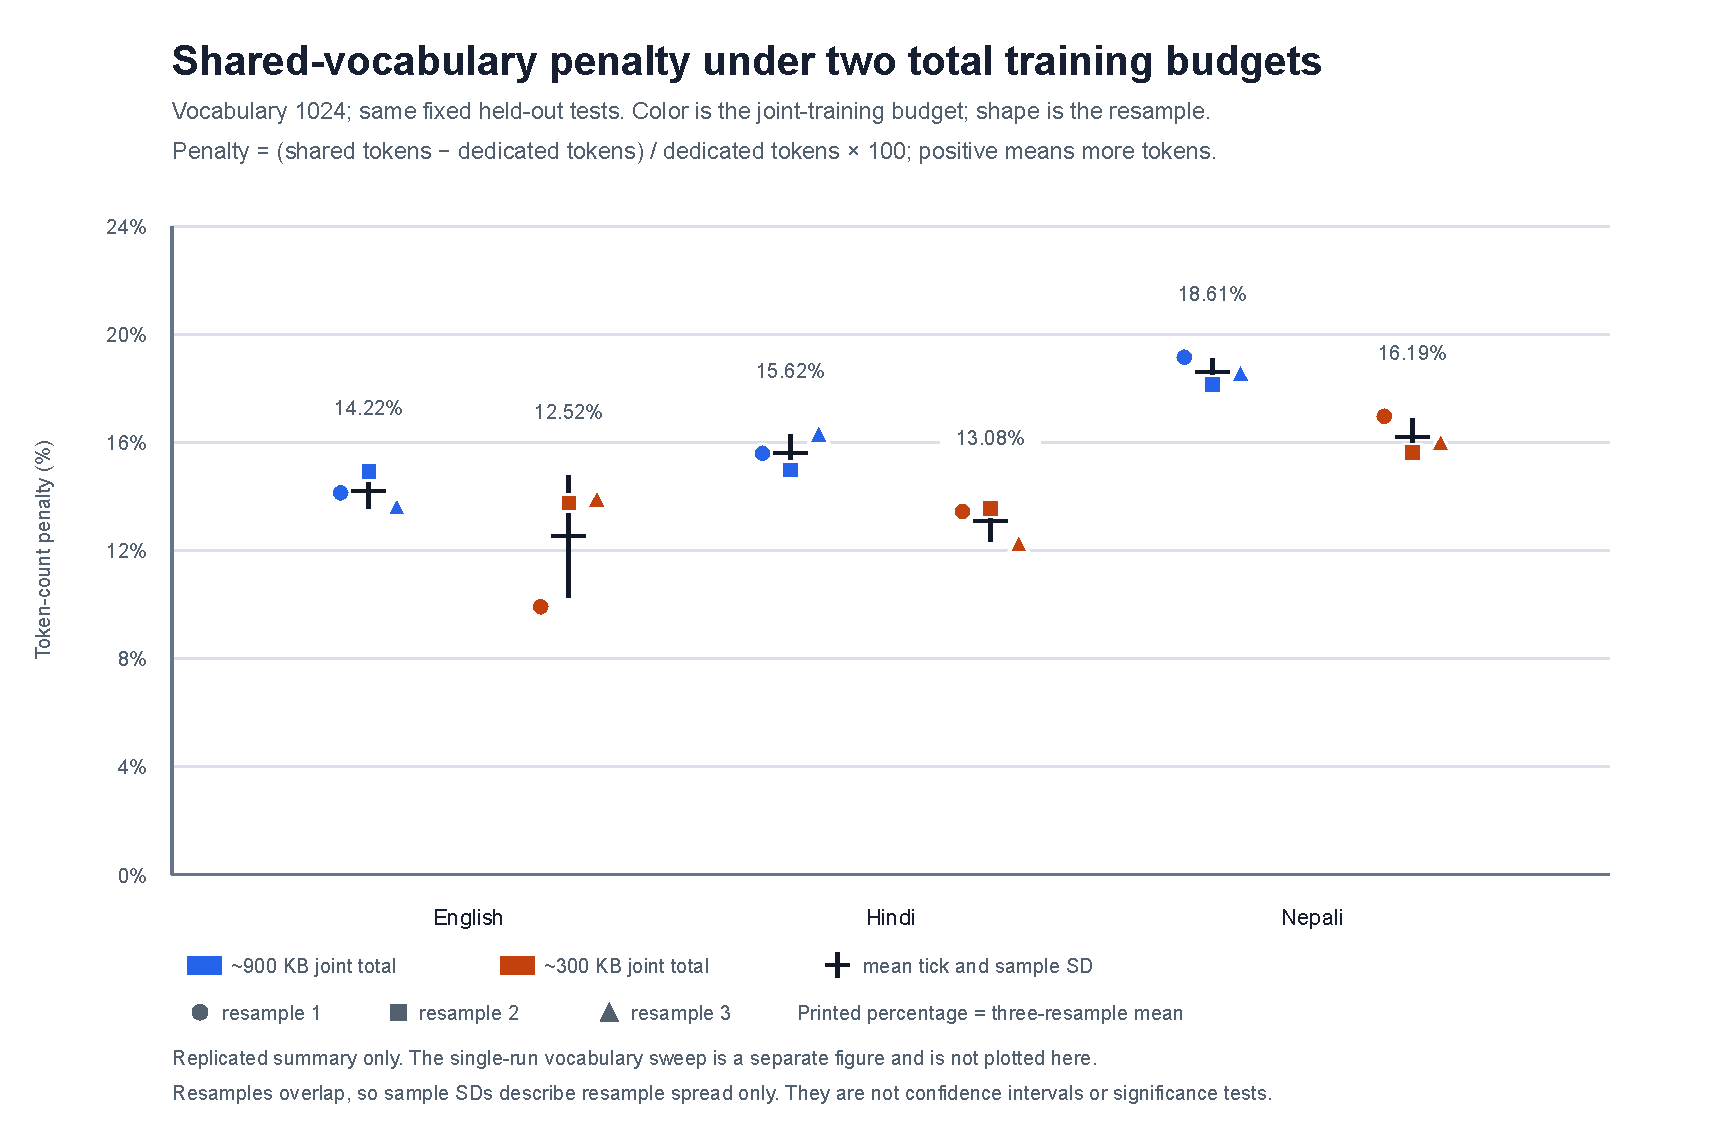
\includegraphics[width=0.98\textwidth]{figures/budget_comparison.pdf}
\caption{Shared-vocabulary penalty at vocabulary 1{,}024 under the two replicated budgets. Points are the three saved resamples. The number is their mean, and the bar is the sample standard deviation. The single-run vocabulary sweep is a separate tier and is not shown. Overlapping resamples make the standard deviations descriptive.}
\label{fig:budgets}
\end{figure*}

\subsection{Percentage penalties and absolute token counts}

The matched-budget means are lower than the fixed-per-language means by about 1.69, 2.54, and 2.42 percentage points.
Table~\ref{tab:absolute} shows why that decrease should not be read as a more efficient joint tokenizer.
The arithmetic mean of the three token counts is higher in the matched regime for every language and for both the dedicated and the joint condition.
Dedicated English token counts rise from a three-replicate mean of 35{,}363.33 to 36{,}851.67, while joint counts rise from 40{,}390.33 to 41{,}462.33.
Hindi moves from 44{,}383.33 to 46{,}014.67 dedicated and from 51{,}317.33 to 52{,}032.00 joint.
Nepali moves from 53{,}641.00 to 55{,}872.00 dedicated and from 63{,}625.33 to 64{,}919.67 joint.
The dedicated denominator grows by more, in relative terms, than the joint numerator, so the ratio falls while both encodings lengthen.

\begin{center}
\footnotesize
\setlength{\tabcolsep}{3pt}
\begin{tabular}{@{}lrrrr@{}}
\toprule
 & \multicolumn{2}{c}{About 300k bytes each} & \multicolumn{2}{c}{Matched subsets} \\
\cmidrule(lr){2-3}\cmidrule(lr){4-5}
Language & Dedicated & Joint & Dedicated & Joint \\
\midrule
English & 35{,}363.33 & 40{,}390.33 & 36{,}851.67 & 41{,}462.33 \\
Hindi & 44{,}383.33 & 51{,}317.33 & 46{,}014.67 & 52{,}032.00 \\
Nepali & 53{,}641.00 & 63{,}625.33 & 55{,}872.00 & 64{,}919.67 \\
\bottomrule
\end{tabular}
\captionof{table}{Mean held-out token counts across the three replicates. The joint column in the first pair is the model trained on about 900{,}000 bytes. The joint column in the second pair is the model trained on about 300{,}000 bytes.}
\label{tab:absolute}
\end{center}

\section{Discussion}

The three research questions have direct answers in the saved runs.
Under a shared cap of about 300{,}000 bytes per language, the joint 1{,}024-token vocabulary uses more held-out tokens than the dedicated vocabulary in all nine comparisons.
The same is true when both conditions use the same 100{,}000-byte subsets.
In the one balanced selection, the penalty is positive at 512, 1{,}024, and 2{,}048 for all three languages.
Those statements are limited to this corpus, this trainer, these budgets, and this metric.

The budget comparison supports a narrower conclusion than a causal claim about data volume.
Moving from the first regime to the second changes the dedicated sample, the joint sample, and which documents appear.
The joint model sees less text, and the dedicated model sees less text as well.
The percentage gap narrows while both token counts grow.
A design that held the dedicated data fixed and changed only the joint budget was not run.

Shared Devanagari orthography did not remove the penalty for Hindi and Nepali.
Nepali has the largest mean penalty in both replicated regimes.
This sample cannot separate script, morphology, web-register mix, and the small document counts.
The saved manifests record 35, 28, and 29 English documents in the three 300{,}000-byte selections, and 12, 10, and 9 English documents in the matched subsets.
The English matched-budget sample standard deviation is 2.26 percentage points.
With so few documents, which lines are kept can change the penalty.
This design does not separate that sensitivity from the other differences among the resamples.

The result sits beside, and does not replace, studies that allocate vocabulary or measure task quality \citep{chung-etal-2020-improving,liang-etal-2023-xlm,brahma-etal-2026-multilingual,ali-etal-2024-tokenizer}.
A tokenizer that uses more tokens can still help or hurt a downstream model.
We did not train one.

\FloatBarrier
\subsection{Limitations}

The source stream is unpinned, so the processed files cannot be assumed to reappear from the dataset name alone.
The audit does not establish provenance or the absence of pre-split contamination.
Resamples overlap, and three is too small a set for a significance claim even if they did not.
The sweep selector and the resample selector do not implement the byte cap in exactly the same way, although both saved files are reported with exact byte counts.
The matched control exists only at vocabulary 1{,}024.
At that size the shared condition uses one 1{,}024-entry vocabulary, and the three dedicated tokenizers collectively use 3{,}072 vocabulary entries.
The experiment matches vocabulary size per tokenizer, not aggregate vocabulary capacity.
The results characterize that specific comparison.
They do not isolate the effect of sharing under an equal aggregate vocabulary budget, because no such condition was trained.
Grapheme and akshara tokenization are outside the main comparison.
No downstream, transfer, or morphological evaluation was run.
The tables can be recomputed from the saved result JSON.
The training scripts refuse to overwrite an existing output, and both the byte-level trainer and the reporting script use the Python standard library.
The package metadata requires Python 3.12.
The held-out files shared by every tier are the processed test splits named in the manifest, with the byte counts in Table~\ref{tab:pool}.

\section{Conclusion}

On this English, Hindi, and Nepali sample, a fully shared byte-level BPE vocabulary of 1{,}024 tokens encodes held-out text with more tokens than a dedicated vocabulary of the same requested size.
The penalty appears in every saved resample when each language supplies about 300{,}000 training bytes, and it remains when dedicated and joint training use the same subsets of about 100{,}000 bytes.
The second setting has a smaller percentage penalty and a larger absolute token count for both models.
That pattern is a reproducible intrinsic token-count comparison for this English--Hindi--Nepali corpus, this byte-level BPE implementation, and these training budgets.
It is not a general law of multilingual tokenization, and it is not evidence about downstream quality.

\section*{Ethics and data}

The text is web data distributed through the named Hugging Face dataset.
The dataset card states a CC0 license and points to HPLT~3.0 as an upstream source.
This study did not independently audit the license, take-down status, or personal information in the saved lines.
The experimental subset is small and is used only to count tokenizer output.
The code, manifests, model files, and result JSON needed to recompute the tables are in the project directory.
Retraining is unnecessary for the numbers in this paper and is blocked by the training scripts when an output file already exists.

\bibliography{references}

\end{document}
